\documentclass{report}
\usepackage[margin=1in]{geometry}
\usepackage{tikz}
\usepackage{pgfplots}
\usepackage[hidelinks]{hyperref}
\usepackage{longtable}
\usepackage{enumitem}
\usepackage{array}
\usepackage{graphicx}
\usepackage{caption}
\usepackage{booktabs}
\usepackage{float}
\usepackage{adjustbox}
\usepackage{datetime2}

% ============================================================================
% CUSTOM DATE STYLE (DD.MM.YYYY)
% ============================================================================
\DTMnewdatestyle{CustomDateStyle}%
{%
  \renewcommand{\DTMdisplaydate}[4]{%
  \number##3.%               % Day
  \DTMtwodigits{##2}.%       % Month
  \number##1%                % Year
  }%
  \renewcommand{\DTMDisplaydate}{\DTMdisplaydate}%
}
\DTMsetdatestyle{CustomDateStyle}

\usetikzlibrary{shapes,arrows.meta,positioning}
\pgfplotsset{compat=1.18}
\title{\textbf{Painting Fever}\\ Technical Design Document}
\begin{document}
\begin{figure}
	\centering
	\includegraphics[width=6cm]{"../Assets/Sprites/Logos/BZ-Interactive-Logo.png"}
\end{figure}
\begin{figure}
	\centering
	\includegraphics[width=8cm]{"../Assets/Sprites/Icons/icon_painting_fever.png"}
\end{figure}
%\enlargethispage{-5cm}
%\vspace{-5cm}
\author{\textbf{BZ-Interactive} \\ Barkın Zorlu }
\maketitle

% Revision History
\section*{Revision History}
\begin{longtable}{|l|l|l|p{9cm}|}
	\hline
	\textbf{Date} & \textbf{Version} & \textbf{Author} & \textbf{Change Description}                                                                                                             \\
	\hline
	28.02.2026    & 0.1              & Barkın Zorlu  & Initial creation of TDD document.                                                                                                       \\
	\hline
	01.03.2026    & 0.2              & Barkın Zorlu  & Expanded system architecture, added detailed class diagrams, documented audio integration, and outlined future painting logic.          \\
	\hline
	01.03.2026    & 0.3              & Barkın Zorlu  & Comprehensive expansion: added input/controls, GUI system, obstacle types, event system, settings, and level progression documentation. \\
	\hline
	23.03.2026    & 0.4              & Barkın Zorlu  & Added Win Menu and Fail Menu documentation, Pop Effect system, BPM-based beat synchronization for lane switching, and related particle effects. \\
	\hline
	23.03.2026    & 0.5              & Barkın Zorlu  & Updated Folder and File Structure. \\
	\hline
	23.03.2026    & 0.6              & Barkın Zorlu  & Updated Organization ICON and Added Game Icon to TDD. \\
	\hline
	23.03.2026    & 0.7              & Barkın Zorlu  & Update TDD with target framerate and planned input customization. \\
	\hline
\end{longtable}
\newpage

\tableofcontents
\newpage

% Executive Summary
\chapter{Executive Summary}
\section{Project Overview}
Painting Fever is a 2D endless-runner style game developed in Godot 4.5 using C\#. The player controls a character that runs forward automatically, switching between two lanes while avoiding obstacles. The core unique mechanic involves painting the environment in sync with music BPM.

\section{Technical Stack}
\begin{itemize}[noitemsep]
	\item \textbf{Engine}: Godot 4.5.1 (C\# / .NET)
	\item \textbf{Rendering}: Forward Plus (2D)
	\item \textbf{Resolution}: 1280x720 (borderless, stretch mode: canvas\_items)
	\item \textbf{Architecture}: Singleton-based service locator pattern with event-driven communication
\end{itemize}

% System Architecture
\chapter{System Architecture}
\section{Game Tree Overview}
The runtime scene hierarchy is deliberately flat to minimise lookup costs. The most important nodes are:
\begin{itemize}[noitemsep]
	\item \texttt{GameManager} – singleton managing state transitions.
	\item \texttt{GUI} – a \texttt{CanvasLayer} that stays on top.
	\item \texttt{GameSceneRoot} – container for all dynamic level nodes.
	\item \texttt{SoundManager} – global audio controller.
	\item \texttt{AudioStreamPlayer} nodes attached to \texttt{SoundManager}.
\end{itemize}

\section{Singleton Dependencies}
\begin{figure}[H]
	\centering
	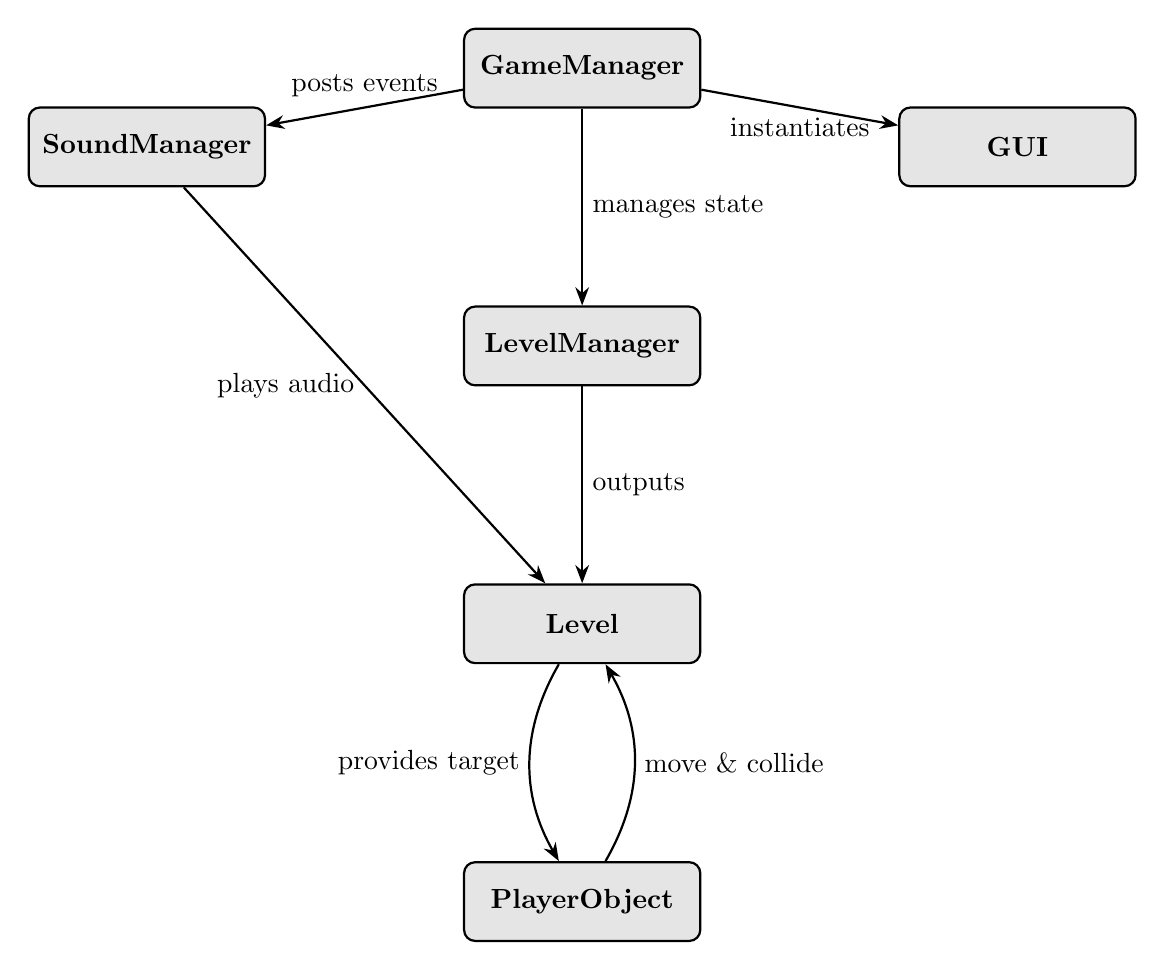
\begin{tikzpicture}[node distance=2.5cm, auto, thick,
			class/.style={rectangle, rounded corners, draw=black, fill=gray!20, minimum width=3cm, minimum height=1cm, align=center}]

		% Nodes
		\node[class] (GM) {\textbf{GameManager}};
		\node[class] (SM) [left=of GM, yshift=-1cm] {\textbf{SoundManager}};
		\node[class] (GUI) [right=of GM, yshift=-1cm] {\textbf{GUI}};
		\node[class] (LevelMgr) [below=of GM] {\textbf{LevelManager}};
		\node[class] (Level) [below=of LevelMgr] {\textbf{Level}};
		\node[class] (Player) [below=of Level] {\textbf{PlayerObject}};

		% Dependencies
		\draw[-Stealth] (GM) to node[above]{posts events} (SM);
		\draw[-Stealth] (GM) to node[right]{manages state} (LevelMgr);
		\draw[-Stealth] (GM) to node[below]{instantiates} (GUI);
		\draw[-Stealth] (LevelMgr) to node[right]{outputs} (Level);
		\draw[-Stealth] (Level) to [bend right=30] node[left]{provides target} (Player);
		\draw[-Stealth] (Player) to [bend right=30] node[right]{move \& collide} (Level);
		\draw[-Stealth] (SM) to node[left]{plays audio} (Level);
	\end{tikzpicture}
	\caption{Core class relationships}
	\label{fig:class_diagram}
\end{figure}
\newpage

% Data Flow
\section{Data Flow Diagram}
\begin{figure}[H]
	\centering
	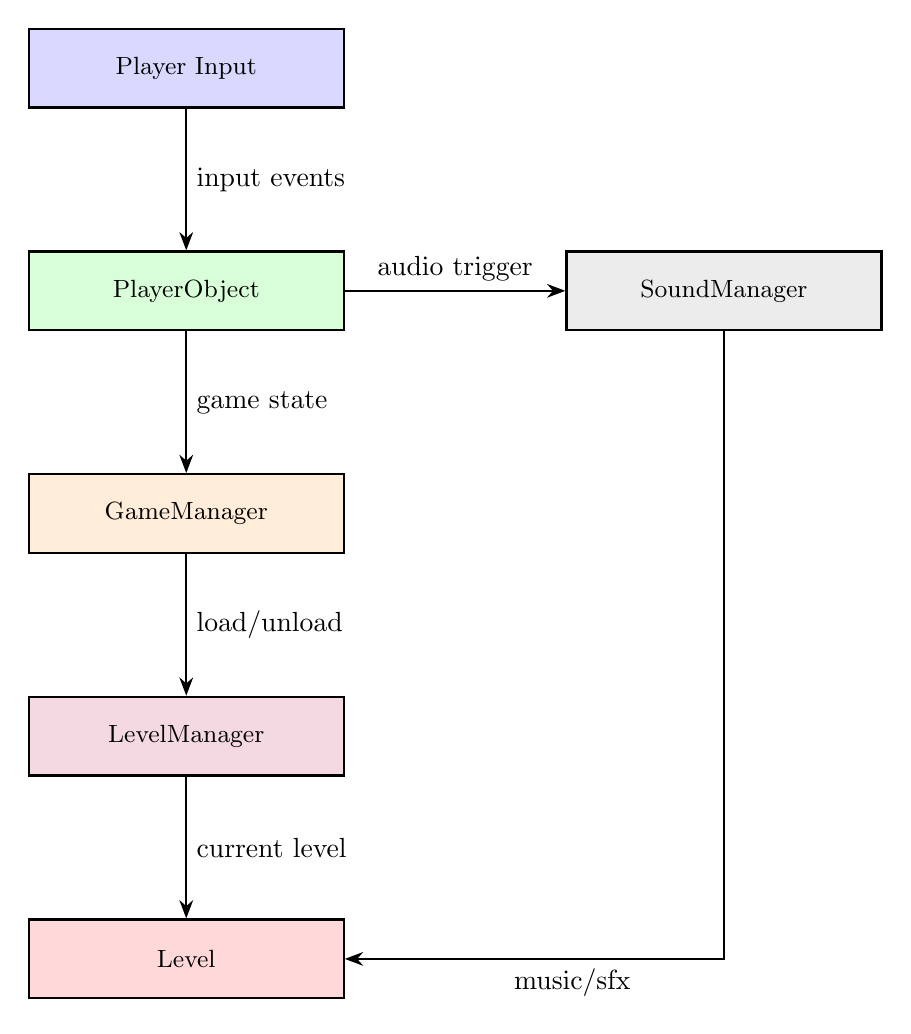
\begin{tikzpicture}[
			node distance=1.8cm,
			auto,
			thick,
			block/.style={rectangle, draw, minimum width=4cm, minimum height=1cm, align=center, font=\small}
		]
		\node[block, fill=blue!15] (Input) {Player Input};
		\node[block, fill=green!15, below=of Input] (Player) {PlayerObject};
		\node[block, fill=orange!15, below=of Player] (GameMgr) {GameManager};
		\node[block, fill=purple!15, below=of GameMgr] (LevelMgr) {LevelManager};
		\node[block, fill=red!15, below=of LevelMgr] (Level) {Level};

		\node[block, fill=gray!15, right=of Player, xshift=1cm] (SoundMgr) {SoundManager};

		\draw[-Stealth] (Input) -- node[right] {input events} (Player);
		\draw[-Stealth] (Player) -- node[right] {game state} (GameMgr);
		\draw[-Stealth] (GameMgr) -- node[right] {load/unload} (LevelMgr);
		\draw[-Stealth] (LevelMgr) -- node[right] {current level} (Level);

		\draw[-Stealth] (Player) -- node[above] {audio trigger} (SoundMgr);

		\draw[-Stealth] (SoundMgr.south) |- node[pos=0.7, below] {music/sfx} (Level.east);

	\end{tikzpicture}
	\caption{Runtime data flow (Vertical Architecture)}
	\label{fig:data_flow_vertical}
\end{figure}

\section{Autoload Nodes}
The project uses Godot's autoload system for global services:
\begin{longtable}{|l|l|p{8cm}|}
	\hline
	\textbf{Node}   & \textbf{Type} & \textbf{Purpose}                           \\
	\hline
	Intro           & Scene         & Boot splash/intro sequence                 \\
	\hline
	SettingsManager & Script        & Global settings persistence and management \\
	\hline
\end{longtable}

\chapter{Input \& Controls}
\section{Input Map Configuration}
All player inputs are defined in \texttt{project.godot} under the \texttt{[input]} section:

\begin{longtable}{|l|l|p{6cm}|}
	\hline
	\textbf{Action}      & \textbf{Keys} & \textbf{Purpose}                         \\
	\hline
	Move Up              & W, Up Arrow   & Switch to upper lane (flip gravity down) \\
	\hline
	Move Down            & S, Down Arrow & Switch to lower lane (flip gravity up)   \\
	\hline
	Color 1              & 1             & Select Red paint color                   \\
	\hline
	Color 2              & 2             & Select Green paint color                 \\
	\hline
	Color 3              & 3             & Select Blue paint color                  \\
	\hline
	Pause                & Escape        & Toggle pause menu                        \\
	\hline
	debug\_reload\_level & R             & Restart current level (DEBUG only)       \\
	\hline
\end{longtable}

\section{Input Handling Patterns}
\begin{itemize}[noitemsep]
	\item \textbf{Movement}: Processed in \texttt{PlayerObject.\_Input()} - lane switching uses gravity flip mechanism
	\item \textbf{Color Selection}: Direct color state change on \texttt{IsActionPressed} events
	\item \textbf{Pause}: Checked via \texttt{GUI.Instance.PauseMenuOpened} to prevent input passthrough
	\item \textbf{Debug}: Conditional compilation (\texttt{\#if DEBUG}) prevents release builds from accessing debug features
	\item \textbf{Frame Rate Target}: Minimum 60 FPS to minimize input latency and ensure responsive rhythm-based mechanics
\end{itemize}

\section{Planned Control Customization}
\begin{itemize}[noitemsep]
	\item \textbf{Remappable Controls}: Future implementation planned for rebindable keybinds if deemed worth.
	\item \textbf{Storage}: User-defined mappings will be persisted via \texttt{SettingsManager}
\end{itemize}

\chapter{Detailed Class Descriptions}
\section{GameManager (\texttt{GameManager.cs})}
\begin{enumerate}[label=\alph*)]
	\item\textbf{Singleton pattern}: accessible via \texttt{GameManager.Instance}.
	\item\textbf{State machine}: \texttt{GameState} enum values control flow; events surface transitions.
	\item\textbf{GUI initialization}: asynchronous root injection after a short timer.
	\item\textbf{State change handling}: broadcasts \texttt{GameStateChanged} and updates internal \texttt{CurrentGameState}.
	\item\textbf{Scene management}: maintains reference to \texttt{GameSceneRoot} for level instantiation.
	\item\textbf{Menu integration}: provides \texttt{ReturnToMainMenu()} for level failure/restart scenarios.
\end{enumerate}

\subsection{GameState Enum}
\begin{verbatim}
public enum GameState
{
    Start,    // Initial state before menu
    Menu,     // Main menu displayed
    Loading,  // Level loading in progress
    Play,     // Active gameplay
    Paused,   // Pause menu open
    End       // Level ended (success/fail)
}
\end{verbatim}

\section{LevelManager (\texttt{LevelManager.cs})}
\begin{enumerate}[label=\alph*)]
	\item\textbf{Level data lookup}: selects packed scenes per \texttt{Difficulty}.
	\item\textbf{Debug reload}: feature active in DEBUG builds, re-instantiates current level.
	\item\textbf{Event hooks}: \texttt{LevelLoaded} and \texttt{LevelUnloaded} for external reactions.
	\item\textbf{Runtime container}: manages \texttt{CurrentLevel} under \texttt{GameSceneRoot}.
	\item\textbf{Level instantiation}: creates levels dynamically based on difficulty and index.
	\item\textbf{Restart capability}: \texttt{RestartCurrentLevel()} preserves current difficulty/index.
	\item\textbf{Time scale management}: maintains \texttt{PausedTimeScale} for slow-motion effects.
\end{enumerate}

\section{Level (\texttt{Level.cs})}
\begin{enumerate}[label=\alph*)]
	\item\textbf{Metadata}: thumbnail, difficulty, distance limits (MaxDistance, RequiredProgress).
	\item\textbf{Music}: audio stream and BPM for beat synchronization.
	\item\textbf{Player injection}: on enter tree, grabs \texttt{PlayerObject} child, configures via \texttt{SetLevelBasedVariables}.
	\item\textbf{Progress tracking}: \texttt{UpdateProgress} records travel and painting status.
	\item\textbf{Level completion logic}: \texttt{CheckLevelEnd} compares distance and required progress.
	\item\textbf{Central line}: \texttt{CentralLinePoint} marker defines the lane center for player positioning.
	\item\textbf{Lane offset}: configurable spacing between the two playable lanes.
\end{enumerate}

\section{PlayerObject (\texttt{PlayerObject.cs})}
\begin{enumerate}[label=\alph*)]
	\item\textbf{Movement}: constant forward speed (X-axis), lane switching via gravity flip (Y-axis).
	\item\textbf{BPM-based lane switching}: lane transitions only succeed when synced with music BPM via \texttt{SoundManager.CheckTiming()}.
	\item\textbf{Collision handling}: triggers level failure on trap layers (collision layer 3).
	\item\textbf{Death effects}: pop particle effect and sound playback on collision via \texttt{PopEffect} and \texttt{PopSound}.
	\item\textbf{Color selection}: interacts with GUI through input actions (1, 2, 3 keys).
	\item\textbf{Painting flag}: \texttt{AbleToPaint} indicates when player is in paint mode (placeholder for future).
	\item\textbf{Stuck detection}: monitors velocity to detect if player has stopped moving forward.
	\item\textbf{Sticky area integration}: responds to \texttt{StickyArea} slowdown effects.
	\item\textbf{Teleportation}: \texttt{TeleportToLocation()} for portal/zone transitions.
	\item\textbf{Gravity direction}: controlled by lane position (positive = down lane, negative = up lane).
\end{enumerate}

\subsection{Player Physics Constants}
\begin{longtable}{|l|l|p{6cm}|}
	\hline
	\textbf{Constant} & \textbf{Value} & \textbf{Purpose}             \\
	\hline
	OBJECT\_RADIUS    & 20.0f          & Player collision radius      \\
	\hline
	GRAVITY           & 9.81f          & Vertical movement multiplier \\
	\hline
	POP\_TIME          & 0.5f           & Pop effect duration in seconds \\
	\hline
\end{longtable}

\section{SoundManager (\texttt{SoundManager.cs})}
\begin{enumerate}[label=\alph*)]
	\item\textbf{AudioServer utilization}: underlying Godot audio engine; all \texttt{AudioStreamPlayer}'s are routed through it.
	\item\textbf{Volume management}: master, music, and SFX volumes with linear-to-dB conversion.
	\item\textbf{Playback control}: dedicated methods for music, SFX, track switching.
	\item\textbf{Settings integration}: pulls user preferences from \texttt{SettingsManager} and applies via events.
	\item\textbf{State-based music}: automatically switches to menu music on state transition to \texttt{GameState.Menu}.
	\item\textbf{Beat timing}: \texttt{CheckTiming(bool printValues)} provides BPM-synchronized input validation for rhythm-based mechanics, with latency compensation via \texttt{AudioServer}.
\end{enumerate}

\subsection{Audio Players}
\begin{longtable}{|l|p{8cm}|}
	\hline
	\textbf{Player}  & \textbf{Purpose}                                         \\
	\hline
	MenuMusicPlayer  & Background music for main menu                           \\
	\hline
	LevelMusicPlayer & Level-specific background music with BPM sync capability \\
	\hline
	EffectsPlayer    & One-shot sound effects (footsteps, collisions)           \\
	\hline
\end{longtable}

\chapter{GUI System}
\section{Architecture Overview}
The GUI system uses a \texttt{CanvasLayer} to remain above all game content. The \texttt{GUI} class acts as a container and state coordinator:

\begin{figure}[H]
	\centering
	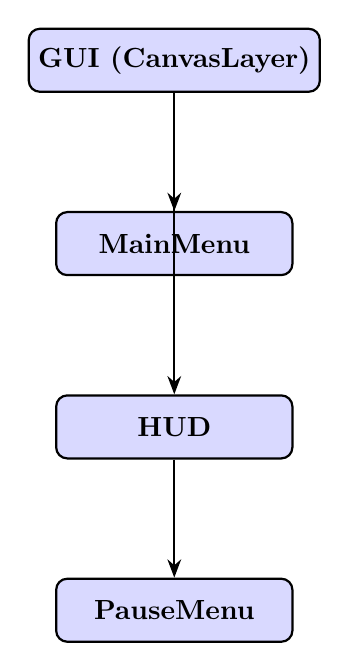
\begin{tikzpicture}[
			node distance=1.5cm,
			auto,
			thick,
			class/.style={rectangle, rounded corners, draw=black, fill=blue!15, minimum width=3cm, minimum height=0.8cm, align=center}
		]
		\node[class] (GUI) {\textbf{GUI (CanvasLayer)}};
		\node[class] (MM) [below=of GUI] {\textbf{MainMenu}};
		\node[class] (HUD) [below=of MM] {\textbf{HUD}};
		\node[class] (PM) [below=of HUD] {\textbf{PauseMenu}};

		\draw[-Stealth] (GUI) to (MM);
		\draw[-Stealth] (GUI) to (HUD);
		\draw[-Stealth] (HUD) to (PM);
	\end{tikzpicture}
	\caption{GUI component hierarchy}
	\label{fig:gui_hierarchy}
\end{figure}

\section{MainMenu (\texttt{MainMenu.cs})}
\begin{itemize}[noitemsep]
	\item Entry point for the game
	\item Contains level selection interface
	\item Links to \texttt{LevelSelector} for difficulty/level picking
\end{itemize}

\section{HUD (\texttt{HUD.cs})}
\begin{itemize}[noitemsep]
	\item In-game heads-up display
	\item Shows current score/progress via \texttt{UpdateProgressBar(float progress)}
	\item Contains references to \texttt{PauseMenu}, \texttt{WinMenu}, and \texttt{FailMenu}
	\item Manages menu visibility and transitions
	\item Toggled visibility based on \texttt{GameState}
	\item Provides \texttt{ShowFailMenu(failReason)} and \texttt{ShowWinMenu(score)} interfaces
\end{itemize}

\section{PauseMenu (\texttt{PauseMenu.cs})}
\begin{itemize}[noitemsep]
	\item Overlay displayed when \texttt{Pause} input is triggered
	\item Pauses game time scale
	\item Provides resume, restart, and quit options
	\item \texttt{Visible} property checked by \texttt{PlayerObject} to block movement input
\end{itemize}

\section{WinMenu (\texttt{WinMenu.cs})}
\begin{itemize}[noitemsep]
	\item Displayed when level completion conditions are met
	\item Shows star rating based on performance score (0-3 stars)
	\item Displays numerical score as percentage
	\item Provides \texttt{NextLevel()} to progress and \texttt{ReturnToMenu()} options
	\item Managed by \texttt{HUD} through \texttt{ShowWinMenu(score)} and \texttt{HideWinMenu()} methods
\end{itemize}

\section{FailMenu (\texttt{FailMenu.cs})}
\begin{itemize}[noitemsep]
	\item Displayed when level failure conditions are triggered
	\item Shows failure reason (e.g., "Out of Bounds!", "Keep up!", etc.)
	\item Provides \texttt{RetryLevel()} to restart current level and \texttt{ReturnToMenu()} options
	\item Manages failure state via \texttt{FailReason} property
	\item Managed by \texttt{HUD} through \texttt{ShowFailMenu(failReason)} and \texttt{HideFailMenu()} methods
\end{itemize}

\section{LevelSelector (\texttt{LevelSelector.cs})}
\begin{itemize}[noitemsep]
	\item Grid-based level selection UI
	\item Displays available levels per difficulty
	\item Uses \texttt{LevelButton} for individual level entries
	\item Organized by \texttt{LevelRow} and \texttt{LevelPage}
\end{itemize}

\chapter{Data Systems}
\section{LevelData (\texttt{LevelData.cs})}
Central configuration resource for all level-related data:

\subsection{Difficulty Speed Mapping}
\begin{longtable}{|l|l|}
	\hline
	\textbf{Difficulty} & \textbf{Move Speed (px/s)} \\
	\hline
	Easy                & 300                        \\
	\hline
	Medium              & 600                        \\
	\hline
	Hard                & 1000                       \\
	\hline
	EasterEgg           & 1000                       \\
	\hline
\end{longtable}

\subsection{Stuck Time Thresholds}
\begin{longtable}{|l|l|}
	\hline
	\textbf{Difficulty} & \textbf{Max Stuck Time (s)} \\
	\hline
	Easy                & 2.0                         \\
	\hline
	Medium              & 1.2                         \\
	\hline
	Hard                & 0.8                         \\
	\hline
	EasterEgg           & 0.8                         \\
	\hline
\end{longtable}

\subsection{Completion Thresholds}
\begin{longtable}{|l|l|}
	\hline
	\textbf{Threshold} & \textbf{Percentage} \\
	\hline
	Passed             & 75\%                \\
	\hline
	Success            & 90\%                \\
	\hline
	Perfect            & 100\%               \\
	\hline
\end{longtable}

\section{ColorData (\texttt{ColorData.cs})}
Stores paint color configurations for the painting mechanic (future implementation).
\pagebreak
\section{Difficulty Enum}
\begin{verbatim}
public enum Difficulty
{
    Easy,
    Medium,
    Hard,
    EasterEgg
}
\end{verbatim}

\section{PlayerColors Enum}
\begin{verbatim}
public enum PlayerColors
{
    Grey,   // Default/neutral color
    Red,    // Paint color 1
    Green,  // Paint color 2
    Blue    // Paint color 3
}
\end{verbatim}

\chapter{Obstacle System}
\section{Trap (\texttt{Trap.cs})}
Static obstacles that cause immediate level failure on collision:

\begin{itemize}[noitemsep]
	\item \textbf{Collision layer}: Layer 3 (designated trap layer)
	\item \textbf{Movement support}: Optional tween-based movement between markers
	\item \textbf{Rotation support}: Configurable rotational animation
	\item \textbf{Transition types}: Linear, Sine, Quad, Cubic, Quart, Quint, Expo, Elastic, Bounce, Back
\end{itemize}

\section{StickyArea (\texttt{StickyArea.cs})}
Area2D-based slowdown zones:

\begin{itemize}[noitemsep]
	\item \textbf{Effect}: Reduces player speed by configurable multiplier
	\item \textbf{Persistence}: Speed gradually restores over 2 seconds after exit
	\item \textbf{Integration}: Uses \texttt{LevelData.stickySlowdownMultiplier} (default: 0.9)
	\item \textbf{State tracking}: Tracks \texttt{Sticked} state on player for external systems
\end{itemize}

\chapter{Event System}
\section{IEventSubscriber Interface}
All event-driven components implement \texttt{IEventSubscriber}:

\begin{verbatim}
public interface IEventSubscriber
{
    void SubscribeToEvents();
    void UnsubscribeFromEvents();
}
\end{verbatim}

\section{Global Events}
\begin{longtable}{|l|l|p{6cm}|}
	\hline
	\textbf{Event}   & \textbf{Parameters}                      & \textbf{Description}                        \\
	\hline
	GameStateChanged & (GameState oldState, GameState newState) & Fired when game state transitions           \\
	\hline
	LevelLoaded      & (Level level)                            & Fired after level instantiation             \\
	\hline
	LevelUnloaded    & (Level level)                            & Fired before level destruction              \\
	\hline
	SettingsChanged  & void                                     & Fired when user settings are modified       \\
	\hline
	GotUnstuck       & void                                     & Fired when player recovers from stuck state \\
	\hline
\end{longtable}

\chapter{Settings System}
\section{SettingsManager (\texttt{SettingsManager.cs})}
Autoloaded singleton from \texttt{BZSettingsSystem} addon:

\begin{itemize}[noitemsep]
	\item Persists user preferences to disk
	\item Provides runtime access via \texttt{Instance.SettingsData}
	\item Broadcasts \texttt{SettingsChanged} on any modification
	\item Integrates with \texttt{SoundManager} for audio preferences
\end{itemize}

\section{SettingsData (\texttt{SettingsData.cs})}
\begin{longtable}{|l|l|}
	\hline
	\textbf{Setting} & \textbf{Default} \\
	\hline
	MasterVolume     & 50               \\
	\hline
	MusicVolume      & 100              \\
	\hline
	EffectsVolume    & 100              \\
	\hline
	ColorBlindMode   & None             \\
	\hline
\end{longtable}

\chapter{Level Progression}
\section{Level Loading Flow}
\begin{enumerate}
	\item Player selects difficulty in \texttt{LevelSelector}
	\item \texttt{LevelManager.InstantiateLevel(difficulty, index)} called
	\item Appropriate \texttt{PackedScene} retrieved from \texttt{LevelData}
	\item Level instantiated under \texttt{GameSceneRoot}
	\item \texttt{Level.\_EnterTree()} triggers player configuration
	\item \texttt{LevelLoaded} event fires
	\item Music begins via \texttt{SoundManager}
\end{enumerate}

\section{Level Completion Logic}
\begin{enumerate}
	\item Player continuously travels forward (X-axis velocity)
	\item \texttt{Level.UpdateProgress()} called each frame with distance and painting status
	\item When \texttt{Distance >= MaxDistance}:
	      \begin{itemize}
		      \item If \texttt{Progress >= RequiredProgress}: Level Success
		      \item Else: Level Failed
	      \end{itemize}
\end{enumerate}

\section{Failure Conditions}
\begin{itemize}[noitemsep]
	\item Collision with \texttt{Trap} (layer 3)
	\item Player exits screen bounds (\texttt{OnScreenExited()})
	\item Stuck for longer than \texttt{MaxStuckTime} (difficulty-dependent)
\end{itemize}

\chapter{Physics Configuration}
\section{Physics Properties}
\begin{longtable}{|l|l|}
	\hline
	\textbf{Setting}           & \textbf{Value} \\
	\hline
	2D Default Linear Damping  & 0.0            \\
	\hline
	2D Default Angular Damping & 0.0            \\
	\hline
\end{longtable}

\section{Lane System}
The game uses a two-lane system:
\begin{itemize}[noitemsep]
	\item \textbf{CentralLinePoint}: Reference marker for lane center
	\item \textbf{LaneOffset}: Distance from center to each lane
	\item \textbf{Gravity flip}: Switching lanes inverts Y-gravity direction
	\item Player Y-position offset by \texttt{OBJECT\_RADIUS} to prevent clipping
\end{itemize}

\chapter{Particle Effects}
\section{Pop Effect (\texttt{pop\_effect.tscn})}
Death/collision particle system triggered when player hits obstacles:

\begin{itemize}[noitemsep]
	\item \textbf{Type}: \texttt{GPUParticles2D} with \texttt{ParticleProcessMaterial}
	\item \textbf{Emitter settings}: 50 particles per emission, 0.4 second lifetime
	\item \textbf{Spread}: 180 degrees for omnidirectional burst
	\item \textbf{Velocity}: 200--500 px/s random initial velocity
	\item \textbf{Physics}: Zero gravity for consistent arc-based motion
	\item \textbf{Visual}: Scale range 1.0--3.0, trail rendering enabled for motion blur
	\item \textbf{Integration}: Attached to \texttt{PlayerObject}, triggered on collision via \texttt{PlayerObject.PopEffect.Emitting = true}
	\item \textbf{Audio coupling}: Plays \texttt{PopSound} simultaneously via \texttt{SoundManager.PlaySfx()}
\end{itemize}

\chapter{Audio Systems}
\section{BPM Synchronization (\texttt{SoundManager.CheckTiming()})}
Beat-accurate input timing for rhythm-based mechanics:

\begin{itemize}[noitemsep]
	\item \textbf{Implementation}: \texttt{SoundManager.CheckTiming(bool printValues)} compares current playback position against nearest beat
	\item \textbf{Calculation}: Seconds Per Beat (SPB) derived from \texttt{Level.MusicBPM}:
	\begin{verbatim}
	SPB = 60.0f / MusicBPM
	\end{verbatim}
	\item \textbf{Precision}: Uses \texttt{AudioServer.GetPlaybackPosition()} for sample-accurate timing
	\item \textbf{Tolerance}: \texttt{Level.MusicOffset} defines acceptable window (in seconds) for beat detection
	\item \textbf{Usage}: Lane switching only succeeds when \texttt{CheckTiming()} returns \texttt{true}, forcing rhythm-based gameplay
	\item \textbf{Debug support}: Optional console output via \texttt{printValues} parameter for tuning offset values
	\item \textbf{Visual feedback}: Performance overlay shows green rect when on-beat, white otherwise
\end{itemize}

\subsection{BPM Configuration per Level}
\begin{longtable}{|l|l|}
	\hline
	\textbf{Property} & \textbf{Description} \\
	\hline
	MusicBPM & Beats per minute of level audio \textit{(required, > 0)} \\
	\hline
	MusicOffset & Acceptable timing window in seconds (default: 0.1s) \\
	\hline
\end{longtable}

\chapter{Future Extensions}
\section{Painting Mesh Generation}
\begin{itemize}[noitemsep]
	\item Current code reserves a \texttt{PlayerObject.AbleToPaint} flag but no mesh creation.
	\item Suggested architecture: a \texttt{MeshBuilder} class that consumes player positions over time, generates segmented polyline meshes and uploads them to a \texttt{MeshInstance2D}. The MeshBuilder would interface with the Level to record progress.
	\item Future audio coupling: passing paint events to \texttt{SoundManager} for beat-synchronized effects.
\end{itemize}

\section{Power-Up System}
Potential future additions:
\begin{itemize}[noitemsep]
	\item Temporary invincibility
	\item Speed boost
	\item Paint multiplier (earn more progress per paint)
	\item Time freeze (slow obstacles temporarily)
\end{itemize}

\section{Portal/Zoning System}
\begin{itemize}[noitemsep]
	\item \texttt{PlayerObject.TeleportToLocation()} exists but needs portal implementation
	\item Would enable non-linear level layouts
	\item Could include zone-specific difficulty modifiers
\end{itemize}

\chapter{Performance Considerations}
\section{Rendering}
\begin{itemize}[noitemsep]
	\item MSAA 2D set to 1 (2x multisampling)
	\item Borderless window with canvas\_items stretch for consistent UI scaling
	\item Scene tree kept shallow to minimize traversal costs
\end{itemize}

\section{Memory Management}
\begin{itemize}[noitemsep]
	\item Levels are unloaded completely via \texttt{QueueFree()} when not in use
	\item Settings loaded once at startup via autoload
	\item No runtime asset loading - all resources bundled at build
\end{itemize}

\chapter{Build Configuration}
\section{Project Settings}
\begin{longtable}{|l|l|}
	\hline
	\textbf{Setting} & \textbf{Value} \\
	\hline
	Engine Version   & Godot 4.5      \\
	\hline
	Language         & C\# (.NET)     \\
	\hline
	Renderer         & Forward Plus   \\
	\hline
	Viewport Width   & 1280           \\
	\hline
	Viewport Height  & 720            \\
	\hline
	Window Mode      & Borderless     \\
	\hline
	Stretch Mode     & canvas\_items  \\
	\hline
	Stretch Aspect   & expand         \\
	\hline
\end{longtable}

\section{Platform Support}
\begin{itemize}[noitemsep]
	\item Primary target: Windows (native icon: \texttt{painting\_fever.ico})
	\item Cross-platform capable via Godot's export system
\end{itemize}

% ============================================================================
% APPENDIX: Quick Reference
% ============================================================================
\appendix
\chapter{Quick Reference}

\section{File Structure}
\begin{verbatim}
Assets/
+-- Scripts/
|   +-- Managers/        (GameManager, LevelManager, SoundManager)
|   +-- Player/          (PlayerObject, physics)
|   +-- Level/           (Level, Obstacles, StickyArea, Trap)
|   +-- GUI/
|   |   +-- Menu/        (MainMenu, PauseMenu, WinMenu, FailMenu)
|   |   |   +-- Levels/  (LevelSelector, LevelButton)
|   |   +-- HUD/         (HUD, progress tracking)
|   |   +-- Intro/       (Intro sequence)
|   |   +-- Overlay/     (PerformanceOverlay)
|   |   +-- Buttons/     (Button components)
|   |   +-- GUI.cs       (Root GUI controller)
|   +-- Data/            (LevelData, ColorData)
|   +-- Enums/           (GameState, Difficulty, PlayerColors)
|   +-- Camera/          (Camera systems)
|   +-- Interfaces/      (IEventSubscriber, etc.)
|   +-- Settings/        (Settings-related scripts)
+-- Scenes/              (Main scene layouts)
|   +-- GUI/             (GUI scene prefabs)
|   +-- Game/            (Gameplay scenes)
|   +-- Intro/           (Intro scenes)
|   +-- main_scene.tscn  (Root scene)
+-- Subscenes/           (Reusable scene components)
|   +-- GUI/
|   +-- Player/
|   +-- Levels/
|   +-- Managers/
|   +-- Obstacles/
|   +-- Camera/
|   +-- Sections/
|   +-- Walls/
+-- Sprites/             (2D graphics)
+-- Music/               (Background and level music)
+-- Sounds/              (Sound effects)
+-- Particle_Effects/    (Particle systems, pop_effect.tscn)
+-- Fonts/               (Custom fonts)
+-- Themes/              (UI themes)
+-- Styles/              (UI style boxes)
+-- Data/                (Asset resources: ColorData.tres, LevelData.tres)
\end{verbatim}

\section{Key Code Locations}
\begin{longtable}{|l|l|}
	\hline
	\textbf{Feature}              & \textbf{File Path}                    \\
	\hline
	Game State Management         & Scripts/Managers/GameManager.cs       \\
	\hline
	Level Instantiation           & Scripts/Managers/LevelManager.cs      \\
	\hline
	Level Configuration           & Scripts/Level/Level.cs                \\
	\hline
	Player Movement \& Input      & Scripts/Player/PlayerObject.cs        \\
	\hline
	BPM Synchronization           & Scripts/Managers/SoundManager.cs      \\
	\hline
	Collision Detection           & Scripts/Level/Obstacle/Trap.cs        \\
	\hline
	Slow-down Effects             & Scripts/Level/Obstacle/StickyArea.cs  \\
	\hline
	Pop Particle Effects          & Particle\_Effects/pop\_effect.tscn    \\
	\hline
	Win Menu                      & Scripts/GUI/Menu/WinMenu.cs           \\
	\hline
	Fail Menu                     & Scripts/GUI/Menu/FailMenu.cs          \\
	\hline
	Pause Menu                    & Scripts/GUI/Menu/PauseMenu.cs         \\
	\hline
	Main HUD                      & Scripts/GUI/HUD/HUD.cs                \\
	\hline
	Level Selector                & Scripts/GUI/Menu/Levels/LevelSelector.cs \\
	\hline
\end{longtable}

% \bibliographystyle{plain}
% \bibliography{references}

\end{document}
